\section{Methodology and Implementation}
% What were the methods used?
% How was the problem designed?
% Driving concepts
% Equations
% Figures

A modular, \acrfull{ABM} approach is ideal for solving complex, coupled,
physics-dependent supply chain problems involving material routing, facility
deployment, and regional and institutional hierarchies. Additionally, the choice to
build \Cyclus on open source libraries in modern programming languages enables
both remote and multiprocess execution on a number of platforms. This section begins by
describing the general design features that make \Cyclus both flexible and powerful:
cluster-ready software and dynamic libraries.  Next, the framework has an
\gls{ABM} paradigm, which provides an expansion in performance beyond typical system dynamics
capabilities, is described, focusing on agent interchangeability and the
implementation of the region-institution-facility hierarchy.
Next, the discrete treatment of objects is discussed in terms of both
resources and materials and time via the \gls{DRE}.
Support for users and developers via the \Cycamore library of
archetypes and the experimental toolkit are also presented.
Lastly, the methods for quality assurance are outlined.

\subsection{Modular Software Architecture}
% Motivation for encapsulated plug-in architecture
% enables ecosystem, ease of contribution across institutions
% enables myriad levels of simulation fidelity
% enables FC analyses that can compare ‘apples to apples'

The architecture of \Cyclus allows developers
to define nuclear fuel cycle agents and processes independent of the simulation
logic. To achieve this, agents are developed using the \Cyclus framework \gls{API}, a set of functions and protocols
which
assist in agent development and specify how agents should be defined.
This encapsulated `plug-in'
design choice provides two major benefits. First, analysts across research institutions can take advantage of the
simulation logic \gls{API} and archetype ecosystem when they apply \Cyclus to
their specific problem. This
mend-and-extend paradigm, common in modern software development, reduces
maintenance overhead and improves software robustness by protecting the core logic
from changes in the extensions.
The researcher can focus on creating or customizing nuclear
facility, institution, resource, and toolkit models within their specific area
of technical expertise. This extensibility, magnified by an open source
development process, frees the community of users to contribute desired
features, independent from the team of \Cyclus core developers.
Second, because \Cyclus uses a modular archetype approach, comparing two
archetypes is straightforward. For example, if an analyst would like
to compare the effect of using different models to determine the input fuel
composition for fast reactors, a variety of fuel fabrication archetypes can be
developed and interchanged while keeping the rest of the fuel cycle fixed
 to compare fuel fabrication designs.

\subsubsection{Cluster-Ready Software}

Groundbreaking insights and new classes of problems can be investigated by
leveraging modern massive computing resources.
However, many fuel cycle simulators rely on \gls{COTS} and Windows-only software that limits
performance on and compatibility with resource computing infrastructures. This
severely constrains the possible scope of simulations and increases the wall-clock time necessary to conduct parameterized sensitivity
analyses and other multi-simulation studies. \Cyclus, on the other hand, is
primarily written in \texttt{C++} and relies on
libraries supported by Linux and UNIX (including Ubuntu and OSX) platforms,
which are flexible and support parallelization.
Furthermore, the core infrastructure and related archetypes are free and
open source, BSD-3-clause licensed. No part of \Cyclus is proprietary or based
on \gls{COTS}, Windows-only software. \Cyclus can therefore be easily deployed
on large computer systems, such as \gls{HTC} systems.

Cyclopts \cite{gidden_cyclopts_2015}, a proof of principle design and
implementation of \Cyclus on such a large computer system, uses UW-Madison's
HTCondor \gls{HTC} infrastructure to perform sensitivity studies on \Cyclus'
resource exchange optimization solvers. To date, it has been used to run over
$10^4$ jobs, or (\TODO{compute time}) total compute hours, using the \Cyclus
library via its resource exchange \gls{API}.  The \gls{HTC} infrastructure has
also been utilized to run and collect information from full \Cyclus simulations
running in parallel on $10^3$ machines reliably for order $10^5$ simulations.

\subsubsection{Dynamically Loadable Libraries}

The \Cyclus architecture encourages efficient, targeted contribution to the ecosystem of
archetype libraries.
With \Cyclus, a researcher can focus on generating an archetype model within their
sphere of expertise while relying on the contributions of others to fill
in the other technologies in the simulation.
Similarly, individual developers may explore different levels of complexity within their archetypes, including
wrapping other simulation tools as loadable libraries within \Cyclus.

\Cyclus acheives this behavior by implementing its generic \gls{API} and
modular architecture via a suite of dynamically loadable plug-in libraries, as
pictured in Figure \ref{fig:framework}.
Though common in modern software architecture, such a plug-in pattern has not
previously been implemented in a nuclear fuel cycle simulator. Dynamically
loadable libraries are the primary mechanism for extending \Cyclus' capability.
This approach provides encapsulation: the core framework operates
independently from the individual plug-in libraries. Thus, any customization or
extension is implemented only in the loadable library.

\begin{figure}[htbp!]
\begin{center}
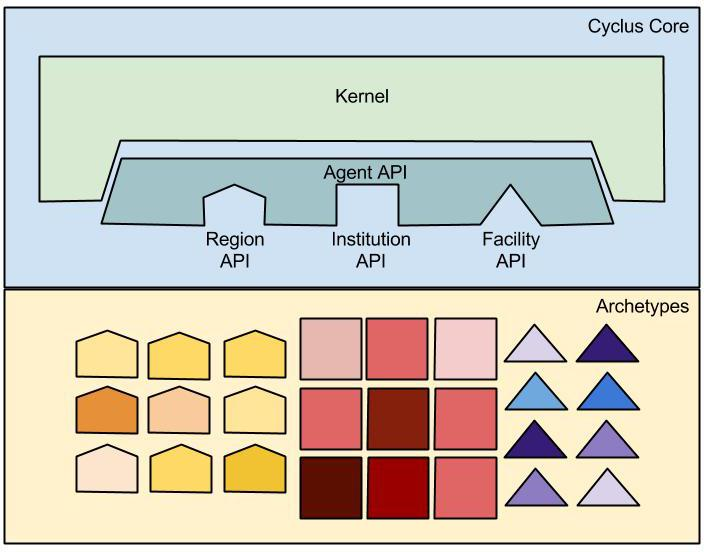
\includegraphics[width=\textwidth]{./images/framework}
\end{center}
\caption{The \Cyclus core provides \gls{API}s that abstract away the details in
the kernel and allow the archetypes to be loaded into the simulation in a modular
fashion.}
\label{fig:framework}
\end{figure}


An additional benefit is the ability for
contributors to choose different distribution and licensing strategies
for their contributions. By allowing models to have varied
availability, the security concerns of developers can be
assuaged (See Figure \ref{fig:modifiedopen}).
In particular, since the clean plug-in architecture loads libraries without any
modifications to the \Cyclus kernel, closed-source archetypes can be used with
the simulator alongside open source archetypes without transfer of sensitive information. This architecture
allows closed-source libraries (e.g., those representing sensitive nuclear
processes and subject to export control) to be developed and licensed privately.

\begin{figure}[htbp!]
\begin{center}
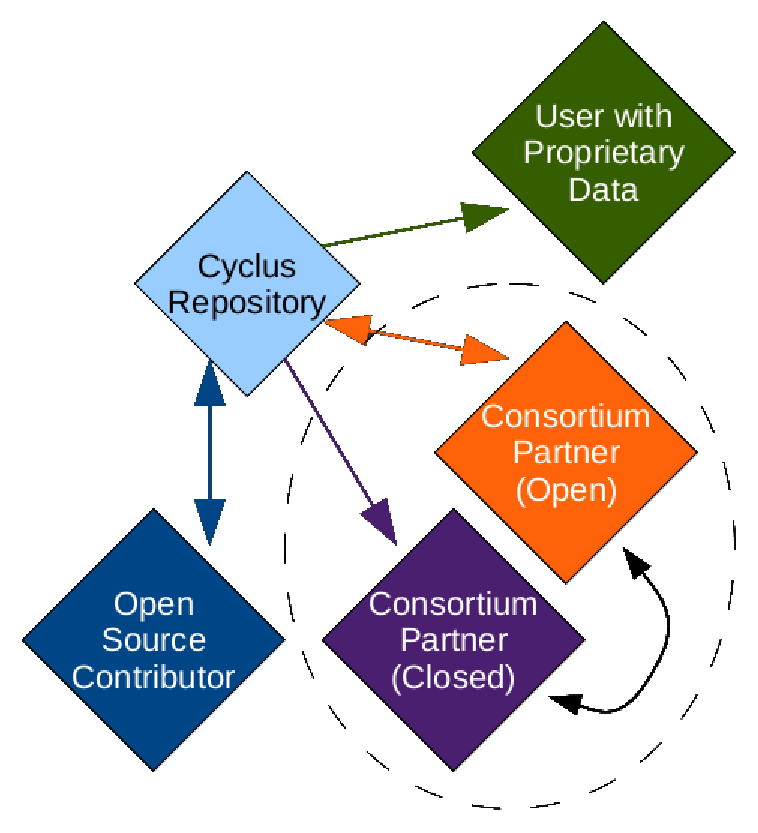
\includegraphics{./images/modifiedopen.eps}
\end{center}
\caption{The \Cyclus framework enables fully open, partially open, and fully
closed collaborations\cite{carlsen_cyclus_2014}.}
\label{fig:modifiedopen}
\end{figure}

This last benefit of dynamically loadable libraries addresses
another goal of \Cyclus: ubiquity amongst its potential user base. By
engineering \Cyclus to easily handle varying levels of complexity, a single
simulation engine can be used by both users interested in big-picture policy
questions as well as users focused on more detailed, technical
analyses. They merely choose their preferred level of fidelity from among the
available libraries in the ecosystem.

\subsection{Agent-based Paradigm}
\label{sec:abm}
% superior detail in capturing simulation dynamics
% more flexible control over behavior
% describe Region/Institution/Facility hierarchy
% note importance of generic resource exchange paradigm

\Cyclus implements an \acrlong{ABM} paradigm.  \gls{ABM} is modern, sophisticated,
true to reality, and incorporates modern computing resources.
Furthermore, \gls{ABM} provides a natural
perspective from which to model a given problem. In the nuclear fuel cycle
context, for example, an analyst can design a reactor agent
that is entirely independent from a fuel fabrication agent. Defining the behavior of both agents according to the
\gls{API} contract is sufficient for them to interact with one another as
bona fide actors in the simulation.  The two archetype libraries can be used in the same
simulation without any shared knowledge.

Furthermore, the \gls{ABM} paradigm is superior to system dynamics used in
current simulators.
System dynamics is a popular approach for modeling nuclear fuel cycles
\cite{jacobson_vision_2009,van_den_durpel_daness_2009,guerin_impact_2009,guerin_benchmark_2009}.
Formally however, system dynamics models are simply a strict subset of agent-based models
\cite{macal_agent-based_2010}.
That is, any system dynamics model can be translated
into an agent-based model. Furthermore, because agent-based
techniques can provide a richer model than can system dynamics, they enable the
broadest range of simulations in a generic fashion.

\subsubsection{Agent Interchangeability}\label{sec:interchangeability}

% (OO, cpp, xml, backends, inheritances, mixins, generic apis, etc.)


\gls{ABM} is inherently object-oriented because agents represent
discrete, independently acting objects.  Figure \ref{fig:framework} illustrates
the modular nature of \Cyclus archetypes.  The core of the \Cyclus simulator
creates a set of classes on which agent plug-ins
are based. In addition, a set of tools are also provided to enrich the
\gls{API} and supply a robust suite of behaviors for the developer.
Agent plug-ins utilize the generic core \gls{API} to interact with one another.  For
example, agents rely on a paradigm of dynamic loading and clean plug-in
behavior at the start of the simulation. They also use the resource exchange
paradigm \gls{API} for trading resources with one another.

Due to this plug-in architecture,
implementations of actors in a given scenario can be easily
interchanged. Critically, this novel functionality enables the comparison
between agent implementations. For example, a low-physics-fidelity
implementation of a reactor can be compared to an implementation with higher
physics fidelity, allowing an analyst to discern the effect of reactor physical
fidelity on a given fuel cycle.

Interchangeability is accomplished by providing \glspl{API} that define agent-to-agent
interaction and agent-to-environment interaction, primarily through the
\Class{Agent} and \Class{Trader} interfaces. Figure \ref{fig:agent_uml} shows
the ``inheritance'' structure of the \Class{Agent} class in a \gls{UML} diagram
format. It shows how the \Class{Agent} interface
provides a notion of parent-child hierarchical relationship, where parents can
choose to \textit{deploy} child agents and \textit{decommission} child
agents. For the archetype developer, this interface provides enormous power
very simply. The \gls{API} provides the \Class{Agent} with helpful functionality for
interacting with the \Cyclus simulation kernel while abstracting away unnecessary
detail.

\begin{figure}[htbp!]
\begin{center}
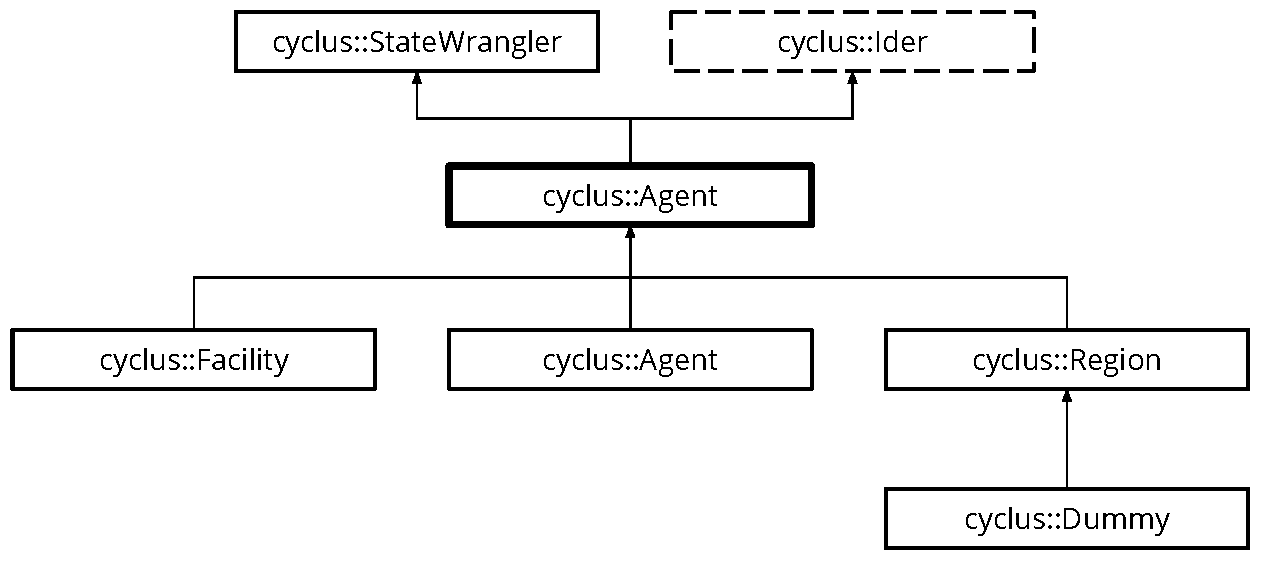
\includegraphics[width=0.5\textwidth]{./images/agent_uml}
\end{center}
\caption{The inheritance in \Cyclus classes, such as the \Class{Agent},
\Class{Facility}, \Class{Institution}, and \Class{Region} classes, abstract away
unnecessary details while exposing powerful functionality. In the above
example, the \Class{Dummy} archetype simply inherits from \Class{Region} in
order to become a bona fide Region-type \Class{Agent}.}
\label{fig:agent_uml}
\end{figure}

In a similar fashion, the \Class{Trader} interface allows agent-agent interaction through the
trading of \Class{Resource}s. Archetypes in a \Cyclus simulation must
implement the \Class{Agent} interface and may optionally implement the
\Class{Trader} interface. For example, a \Class{Region} implements only the
\Class{Agent} interface, whereas a \Class{Facility} implements both the
\Class{Agent} and \Class{Trader} interface, allowing any \Class{Facility} to
trade with another \Class{Facility}.

In this way, a researcher can directly compare two different reactor modeling
implementations (perhaps \Class{DetailedReactor} and \Class{SimpleReactor})
simply by exchanging the two corresponding archetypes. That is, two reactor
archetypes both inheriting from the \Class{Facility} class are indistinguishable
from a simulation perspective. Two simulations, one using
\Class{DetailedReactor} and the other using \Class{SimpleReactor} can therefore
be compared directly to determine the whole-simulation impact of using one or the other model.
This can be done with any agent type, where agents can be ``Regions,''
``Institutions,'' or ``Facilities.''

\subsubsection{Regions, Institutions, and Facilities}

\Cyclus provides a novel representation of entities in the nuclear fuel cycle
that reflects the reality in international nuclear power: production
encompassing facilities, institutions managing those facilities, and regions. While
few simulators have provided any notion of static regional
effects \cite{huff_next_2010,juchau_modeling_2010}, \Cyclus allows for both regions and institutions to be first-class
actors in simulated fuel cycles. The fundamental interactions for each entity are implemented in a corresponding
archetype class in \Cyclus, i.e., the \Class{Region} class, \Class{Institution}
class, and \Class{Facility} class. Archetype developers can then build on the
provided functionality by inheriting from the appropriate class.
\Cyclus implements a \gls{RIF} relationship through the
parent-child hierarchy described in \S \ref{sec:interchangeability}, where
regions are the parents of institutions which are, in turn, the parents of
facilities. In other words, \gls{RIF} hierarchies form a directed acyclic graph (DAG),
with regions as root nodes and facilities as leaf nodes.

Two primary consequences arise from this structure. First, institutions are
nominally
responsible for deploying and decommissioning facilities. Accordingly, advanced
logic regarding building and decommissioning can be obtained by inheriting
those behaviors from the
\Class{Institution} interface. Second, the \Class{Facility} class implements the
\Class{Trader} interface, and thus institutions and regions, respectively, can
adjust the resource flow preferences of their managed facilities. Importantly,
this capability allows for the modeling of preferential regional trading
of resources (e.g., tariffs) as well as preferential institutional trading
(e.g., long-term contracts).

Although concept of the \gls{RIF} hierarchy is provided explicitly, the \Cyclus kernel is
designed to handle hierarchies of arbitrary depth.  It is capable of
running a simulation without regions and institutions (i.e.  only facilities)
or a simulation having archetypes that are the parents of regions.  By
convention, institutions are mainly responsible for facility deployment, but
all archetypes have access to the agent deployment mechanism. \Cyclus enables
the developer to to implement agents that deploy copies of themselves, or that
schedule their own decommissioning.  Because regions, institutions, and
facilities are all just agents, they can all be implemented to exercise the
full set of features offered by the \Cyclus kernel.

\subsection{Discrete Objects}
% enables more realistic models and metrics
% material routing metrics
% shadow fuel cycles
% etc.

\Cyclus models facilities, institutions, regions, and resources as discrete
objects. A discrete resource model allows for a range of modeling granularity. In the
macroscopic extreme, it is equivalent to time-stepped continuous flow. In the
microscopic extreme, the model is capable of representing arbitrarily small
material objects at isotopic resolution. In this way, \Cyclus is
applicable across the full range of modeling extremes.

Fleet-based, lumped-material models do not distinguish between discrete
facility entities or materials. However, some questions require resolution at the level of
individual facilities and materials.
As a result, many detailed performance
metrics cannot be captured with previously existing fleet-based models.

\subsubsection{Resources and Materials}
% Resources, Materials (note isotope tracking, decay behavior)

For all of the reasons that the \gls{ABM} paradigm in \ref{sec:abm} enables
novel simulations, multiple use cases require that these agents, such as the
regions, institutions, and facilities in \Cyclus, must be represented as
discrete objects. Furthermore, important use cases are enabled when materials
and resources are tracked as discrete objects alongside those agents.

One such use case seeks to capture system vulnerability to nefarious
material diversion. Provenance and trade-history of distinct materials is the fundamental
information unit in such studies, and so this type of analysis requires
 discrete simulation of a
target facility and the individual materials modified within it.
Provenance and trade-history of distinct materials is the fundamental
information unit in such studies.
Material risk analysis, therefore, demands that both facilities and materials
should be discretely modeled objects like those in \Cyclus.


In \Cyclus, agents can transfer discrete resource objects among one another.
Cyclus currently supports two types of resources:

\begin{itemize}

  \item Materials: These represent typical nuclear materials with
      nuclide compositions.

  \item Products: These can represent any user-defined measure - e.g. carbon
      credits, build permits, employees, etc.

\end{itemize}

All operations performed on every resource object (splitting, combining,
decay, etc.) are tracked in detail as they are performed.  This information
includes the agent that created each resource when it was introduced into the
simulation.  The parentage of each resource is also tracked. This makes it
possible to follow the history of resources as they are transferred between
agents.  This powerfully impacts the ability to model
non-proliferation-related simulation goals.

The \Cyclus kernel has built-in experimental support for decay calculations.
Materials store the time since their last decay and agents are free to
invoke the decay function on them as desired to decay them to the current
simulation time. \Cyclus can currently operate in 2 decay modes, with 2 additional
modes likely to be added in future releases:

\begin{itemize}

    \item "manual" (currently implemented) is the default mode
        where agents decay materials as needed.

    \item "never" (currently implemented) globally turns off all decay.
        The Material decay function does nothing.

    \item "periodic" (future) automatically decays all materials in a
        simulation with some fixed frequency.

    \item "lazy" (future) decays any material whenever its composition is
        viewed (e.g. when an agent queries information about a material's
        $^{239}$Pu content).

\end{itemize}

In order to avoid excess decay calculations, when decay
is invoked, a material checks to see if it contains any nuclides with decay
constants that are significant with respect to the time change since the last
decay operation.  If none of the decay constants are significant, no decay
calculation is performed and the material remains unchanged.  This error does
not accumulate because the next time the material's decay function is invoked,
the time change will be larger.

\Cyclus has no notion of ``tracked'' versus ``untracked'' nuclides.  In \Cyclus, the composition of a material
is represented by an arbitrarily large list (potentially thousands) of
nuclides.  Agents are free to treat nuclides present in materials any way they
please - including ignoring them.  It is the responsibility of archetype
developers to choose how to handle potentially full-fidelity compositions.

In large simulations, many material objects may change frequently.
Material decay can also contribute significantly to such changes.  In order to
help avoid unnecessary runtime performance and database size impacts,
compositions in \Cyclus have some special features.
Immutability of compositions allows multiple material objects to all hold
references to the same composition object safely.  When operations that do not
alter the composition are performed on a material, any new resulting
materials hold a reference to the same, original composition object.
Although the decay operation generates a new, separate composition (preserving
immutability), a reference to the new composition is placed in a cache shared
by the new and original compositions. The next time the original
composition is decayed, this cache will be checked for a prior calculation
with the same cumulative decay time.  If one exists, the cached composition is
used.  This cache is shared by all compositions that transitively come from
the same origin.  Composition immutability in concert with decay history
caching help eliminate many redundant decay calculations in addition to
reducing the total number of composition objects.  Since each composition
object is only recorded in the database once, significant space savings also
occurs.
\TODO{do we want a diagram helping show this composition caching?}

\subsubsection{Dynamic Resource Exchange}

Since the \Cyclus simulation paradigm involves both discrete agents and
discrete resources, the logic engine defining resource interaction mechanisms
among agents is crucial. The \gls{DRE} is that critical logic engine on which \Cyclus
simulations are built.
As the \Cyclus supply-demand resolution framework,
the DRE must be able to support arbitrary facilities. Supporting the general
\Cyclus philosophy, facilities are treated as black boxes and a clear
supply-demand communication framework is defined.

The \gls{DRE} consists of three steps: supply-demand information
gathering, resource exchange solution, and trade execution. Importantly, each
step is agnostic with respect to the exchange of resources in question, i.e.,
the same procedure is used for both Materials and Products.

The information-gathering step begins by polling potential consumers. Agents
define both the quantity of a commodity they need to consume as well as the
target isotopics, or quality, by posting their demand to the market exchange as
a series of \textit{requests}. Users may optionally parameterize the agent to
associate a collection of demand constraints with each collection of requests.
Collections of requests may be grouped together, denoting \textit{mutual}
requests that represent demand for
some common purpose. For example, a reactor may request \gls{UOX} and \gls{MOX} fuel
mutually, indicating that either will satisfy its demand for fuel.

Suppliers then respond to the series of requests with a \textit{bid}. A bid
supplies a notion of the quantity and quality of a resource to match a
request. Suppliers may add an arbitrary number of constraints to accompany
bids. For example, an enriched \gls{UOX} supplier may supply both a natural uranium
and SWU constraint. Any potential resource transfer may be denoted as
\textit{exclusive}. An exclusive transfer must either be met fully or not at all
in order to support concepts such as the trading of individual reactor
assemblies.

Finally, requesting facilities, institutions and regions may apply
\textit{preferences} to each potential request-bid pairing based on the proposed
resource transfer. Therefore, an institution can apply a higher preference to a
partner to which it is congenial; similarly, a region may negate any transfers
of material which have a higher uranium enrichment than is allowable.

Given a full definition of supply and demand, the \gls{DRE} may be solved either
optimally using a mathematical program or approximately by a simulation-based
heuristic \cite{gidden_agent-based_2014}. If any trade is denoted as exclusive, e.g., if an
analyst desires an assembly-fidelity model, then either a heuristic must be used
or exchanges must be represented as a \gls{MILP}. If no exclusive trades exist,
a \gls{LP} model may be used. In practice, LPs solve much faster than
\gls{MILP}s. However, both capabilities exist in \Cyclus in order to
provide users with the desired level of fidelity.

Trades between agents are initiated by the \Cyclus kernel after a solution to
the \gls{DRE} is found. For each trade, the supplying agent is notified of its
matched request and provides an associated resource to the exchange. All
supplied resources are then sent to the corresponding requesting agents.

In \Cyclus, the \gls{DRE} is executed at each time step. Therefore, if a
facility's request for a resource is not met at a given time step, it may offer
a request in the proceeding time step. Because agent behavior may change
arbitrarily, the exchange executed at any given time step may be unique in a
simulation.

The \gls{DRE} is a novel simulation concept in the nuclear fuel cycle domain. It
provides a flexible supply-demand infrastructure, supporting dynamic flows of
resources between agents. Trading between agents can be affected by both the
proposed quality of a resource and agent relationships through the use of
preferences. Accordingly, a wide range of possible effects can be
modeled, from capacitaty-limited fuel supply to international trade agreements.

\subsection{Simulation Support}
So that users and developers can build working simulations
in the shortest time possible, the \Cyclus ecosystem provides the fundamental
building blocks: basic archetypes and a toolkit of commonly needed functions.
The \Cycamore library provides a suite of fundamental Region, Institution, and
Facility archetypes, while the \Cyclus toolkit provides assistance to
developers.

\subsubsection{Cycamore}
% base modules

\Cycamore \cite{carlsen_cycamore_2014}, the \Cyclus additional module
repository, provides a fundamental set of agent archetypes for basic simulation
functionality within \Cyclus.  Since \Cyclus relies on external
archetypes to represent the agents within a simulation, \Cycamore provides the
basic archetypes a new user needs to get started running simple simulations.
These archetypes support a minimal set of fuel cycle simulation goals and
provide, by example, a guide to new developers who would seek to contribute
their own archetypes outside of \Cycamore.

As of version 1.0, \Cycamore contains four facility archetypes, one region
archetype, and two institution archetypes. Short descriptions of these
functions can be found in Table \ref{tab:cycamore}.


\begin{table}[h]
\centering
\begin{tabularx}{\textwidth}{|r|l|X|}
\hline
\textbf{Entity} & \textbf{Archetype} & \textbf{Functionality} \\
\hline
Facility & BatchReactor & A reactor model that handles batch refueling, based on pre-determined recipes of compositions. \\
Facility & Source & This facility generates material of the composition and commodity type specified as input.  \\
Facility & Sink & This facility is capable of accepting a finite or infinite quantity of some commodity produced in the simulation. \\
Facility & EnrichmentFacility & This facility enriches uranium at a specified capacity. \\
Institution & ManagerInst & The manager institution manages production of commodities among its facilities by building new ones as needed. \\
Institution & DeployInst &  This institution deploys specific facilities as defined explicitly in the input file. \\
Region & GrowthRegion & This region determines whether there is a need to meet a certain capacity (as defined via input) at each time step. \\
\hline
\end{tabularx}
\caption{The Archetypes in \Cycamore seek to cover a large range of simple simulation use cases \cite{carlsen_cycamore_2014}.}
\label{tab:cycamore}
\end{table}

The current \Cycamore release provide basic functionality, As illustrated in
Figure \ref{fig:simplesim}, the current \Cycamore release provides basic
functionality enabling simple fuel cycle analyses. As future contributions are
vetted, the capabilities in \Cycamore may grow.

\begin{figure}[htbp!]
\begin{center}
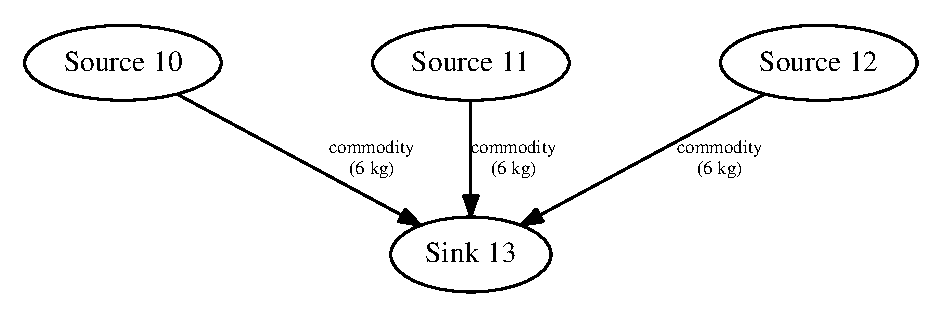
\includegraphics{./images/simplesim}
\end{center}
\caption{Material flows through a simple dynamic simulation created with only the simplest \Cycamore archetypes, \Class{Sink} and \Class{Source}.}
\label{fig:simplesim}
\end{figure}

\subsubsection{Toolkit}

In addition to the core functionality of the \Cyclus kernel, which is focused on
the set of capabilities needed to implement an agent-based simulation
with \gls{DRE}, a toolkit is provided to assist developers
and users with related simulation and nuclear engineering tasks. The toolkit is
an actively developed part of \Cyclus, with a primarily forward-looking
focus on supporting interesting \textit{in situ} metric analysis tools.

\paragraph{Simulation Tools}

A series of utility classes are provided to support demand-constrained agent
facility deployment. For example, symbolic function representations of linear,
exponential, and piecewise functions are supported via the
\Class{SymbFunctionFactory} class. Such functions are used with other toolkit
classes to determine commodity demand (e.g., power demand) from user input. Four
mix-in classes provide the basis for in-simulation deployment determination:
\Class{CommodityProducer}, \Class{CommodityProducerManager}, \Class{Builder},
\Class{BuildingManager}. The \Class{CommodityProducer} class provides an
interface for querying the \textit{prototypes} which have the
capacity to produce a given commdity. The \Class{CommodityProducerManager}
provides an interface for registering \Class{CommodityProducer}s and querying
the current capacity (supply) of a commodity. The \Class{Builder} class provides
an interface for querying which prototypes can be built and interacts with the
\Class{BuildingManager}, which orders prototypes to be built. The
\Class{BuildingManager} uses a simple minimum cost algorithm to determine how
many of each prototype, $y_i$, to build given a demand ($\Phi$), capacities
($\phi_i$), and costs ($c_i$).

\begin{equation}
\begin{aligned}
 \min & \sum_{i=1}^{N}c_i y_i \\
 s.t. & \sum_{i=1}^{N}\phi_i y_i \ge \Phi \\
      & n_i \in [0,\infty) \:\: \forall i \in I, \:\: y_i \:\: \text{integer}
\end{aligned}
\end{equation}

\paragraph{Nuclear Engineering Tools}

The \Cyclus toolkit provides two useful interfaces for querying physical paramaters of \Class{Material}
objects. First, the \Class{MatQuery} module
provides a basic querying \gls{API}, including the atom and mass fractions of
nuclides, the number of moles of a nuclide in a material, and also the amount of
aggregate nuclides, i.e., a \Class{Composition}, in a material. The
\Class{Enrichment} module provides an \gls{API} for determining enrichment-related
parameters of a material, including the separative work units (SWU) and natural
uranium required to enrich a material provided knowledge of feed, product, and tails
assays.

\paragraph{Toolkit Extensions}

In addition to those that already exist, new tools and computational patterns will
emerge from the archetypes developed within the community of
developers. As these tools gain adoption between projects and demonstrate their
utility to the developer community, they will be considered for screening and
adoption into the kernel as toolkit extensions. Likely extensions include

\begin{itemize}
\item fuel cycle metrics calculators,
\item supportive data tables,
\item policy models,
\item and economic models.
\end{itemize}

\subsection{Quality Assurance}
% Organize this section according to major topics
% give each topic a section heading in boldface.
% try to cover the major common points :
%
% problem design
% methods of measurement
% supporting models
% supporting data
% simulations run
% results

% Just write the section headings for each part and indicate what goes in that
% section with words :
%
% heading
% figures (with captions)
% schematics (with captions and footnotes)
% equations
% tables

% What does it mean?
% What did I actually test?
% What were the results?
% Did the work yield a new method?
% Did the work yield new knowledge?
% What measurements did I make?
% How were these measurements characterized?
% What methods were used?
% What were the results?
% How were the measurements made and characterized?

Simulation science - like experimental science - must distinguish trustworthy
results from untrustworthy ones.
Charles Babbage famously articulated this, ``On two occasions I have been asked,
`Pray, Mr. Babbage, if you put into the machine wrong figures, will the right
answers come out?' ... I am not able rightly to apprehend the kind of confusion
of ideas that could provoke such a question.'' \cite{babbage_passages_2011}.
A simulator must assure correctness and guard against the \emph{garbage
in, garbage out} phenomenon.

Multiple strategies, collectively known as \emph{\gls{QA}}, have
been invented to mitigate structural and algorithmic errors
in software. These include \emph{\gls{VV}}
\cite{boehm_software_1989}, \emph{\gls{UQ}}
\cite{sacks_design_1989}, testing, and others.

Nuclear engineering software quality is often governed by \gls{NQA1}, an
\gls{ASME} specification
whose latest revision appeared in 2009 \cite{asme_nqa-1a-2009_2009}.
\Cyclus has adopted an \emph{agile} development process
\cite{larman_agile_2004},
interpreting \gls{NQA1} in a manner similar to the process adopted by the
\gls{DOE} within \gls{NEAMS} \cite{neams_nuclear_2013} or by the PyNE toolkit
\cite{biondo_quality_2014}.

Since \Cyclus modeling decisions are made
by third party archetype developers or users, the most important feature of
\gls{QA} is verification. Validation may be impossible and \gls{UQ} is beyond
the scope of the kernel.

Verification may be defined as the question, ``Is \Cyclus being built correctly?''
To answer this question, \Cyclus relies on software development best practices
such as testing,
documentation, version control, style guidelines, and continuous integration to
ensure reliability and reproducibility. These verification techniques are
discussed individually in the sections that follow.

Validation, in contrast,  may be defined as the question,
``Is \Cyclus the correct tool?''
Since \Cyclus is alone in its class as an agent-based fuel cycle simulator, longitudinal
validation is not possible. Nonetheless, code-to-code comparisons with fuel cycle
simulators that use other modeling paradigms are underway
\cite{huff_extensions_2014}. However, such
exercises are more likely to bring into relief the differences between the modeling
paradigms than supply substantial \gls{QA} and validation.

Lastly, \gls{UQ} is a process that is used on specific simulation
instantiations to statistically determine quality. \gls{UQ} is a process that applies
to the running of many \Cyclus simulations. The kernel itself, as a generic fuel cycle
simulator, cannot make reliable statements about the uncertainty of metrics for a particular fuel
cycle. Any \gls{UQ} results are applicable only to the scenario that is under
analysis by the user. \Cyclus is not a substitute for due diligence on behalf of the fuel
cycle modeler. Thus, \gls{UQ} is envisioned to be beyond the scope of core development
and in the domain of the expert user.

Sections \ref{sec:qa-testing}-\ref{sec:qa-ci} discuss in greater detail the software
development components that comprise the \Cyclus verification strategy.
Each of these on its own is a valuable addition to \gls{QA} but is cannot be the
entire answer to the requirements imposed by \gls{NQA1}. Taken together and strictly
adhered to, they present a fortress to protect against poorly designed or otherwise undesirable code.


\subsubsection{Testing}
\label{sec:qa-testing}

Automated software \emph{testing} is the first line of defense against
errors in implementation. It also acts as an early warning sign if the
simulator does not work as intended on a new system.
Testing serves a critical role in \gls{QA} because it directly compares the
results of running software versus the expected behavior of the software.
In \Cyclus, three categories of tests are defined: unit tests, integration
tests, and regression tests.

It is important to note that before a proposed
code change is allowed into \Cyclus,  the change must be covered by a test, either new or existing, and all of the tests must pass.  This is a
matter of policy for the developers. Of course, test code is
just as likely to contain errors as the code it is designed to test.
However, it is assumed that diligence and one level of testing
is sufficient to meet the aims of \gls{QA} and prevent an infinite recursion
of testing-the-tests.

\paragraph{Unit Tests}

Unit tests compare the results of the smallest code \emph{unit},
typically a single function or a class. What constitutes the smallest code
unit depends on the context of the specific unit in question. While this is
an ambiguous definition, when combined with a philosophy of keeping units as small
as possible, it is often clear in practice what needs to be tested.

\Cyclus uses the Google Test framework \cite{inc_googletest_2008} as a harness for running unit
tests. Sufficient unit tests are required for any proposed change to the \Cyclus
code base. Currently, \Cyclus implements over 450 unit tests and \Cycamore implements
85.  These cover approximately 65\% of their respective code bases, and these numbers are expected to grow over time.

\paragraph{Integration Tests}

Integration tests combine multiple elements of the
\Cyclus interface and test that they work correctly with each other.  By analogy,
simply because the gears (units) are made correctly does not imply that the
clock (integration) will run smoothly, run at all, or give the correct time.
In \Cyclus and \Cycamore, integration tests are performed by running sample
simulations and verifying that results are what would be expected ahead of
time. A set of standard input files have thus been constructed.
Python is used to run the same set of \Cyclus simulations as a subprocess for each integration test.  The results are then inspected and compared via Nose \cite{pellerin_nose_2007}, a Python test framework.
In this way, \Cyclus code units are tested in the full context that they will be
executed. This category of testing is especially useful for ensuring that
major \Cyclus components are functioning as expected.

\paragraph{Regression Tests}

Regression tests ensure unexpected backwards-incompatible changes do not
occur over the course of \Cyclus development. Such a change is called a
\emph{regression} because the new version is almost always wrong.
Regression tests are implemented similarly to integration tests.
Nose is used to execute full \Cyclus simulations whose results
are then compared. In this category, however, the comparison is done against
the output of the same input file when run with a previous version of \Cyclus,
typically the last released version.
In some sense, regression tests are `dumb' in that they do
not care about the contents of a simulation being correct, only whether or not
it changed. They pick up glaring time-sensitive mistakes that may
not appear elsewhere, though they do not purport to make claims about the
quality of the physics modeled. Regression tests are primarily implemented
in \Cycamore because its archetypes are sophisticated enough
to make interesting simulations.

\subsubsection{Documentation}

All of the public interface (the \gls{API}) must be documented as required by the \Cyclus
\gls{QA} policy. This certifies that the intention for a code unit is communicated
in way that is separate from its implementation. This policy is important
because implementations are often wrong and do not reliably communicate their intent. Truly trustworthy communication about what
software should be doing occurs when the author explicitly states the
goals of an \gls{API} in prose form. Future developers are then able to
compare the implementation versus the documentation to discern whether or not
these are in agreement. Documentation is thus a secondary higher-level information
stream.  In \Cyclus, this information is aggregated together into static
websites with the Doxygen \cite{van_heesch_doxygen:_2008} and Sphinx
\cite{brandl_sphinx_2014}
tools, and can be accessed at \url{http://fuelcycle.org}.

\subsubsection{Version Control}

Version control preserves the development history, or \emph{provenance}, of
source code files. \Cyclus uses a well-established \emph{distributed version
control} tool called git \cite{software_freedom_conservancy_git_2014} for this
purpose.  Distributed version control allows every
user to have complete local copy of the \emph{repository} (the version control
term for the collection of all possible histories).
One feature that git performs exceptionally well is \emph{branching}.
Branches are distinct pathways in the history that diverge from a mainline source
tree and then may be \emph{merged} back in. Multiple simultaneous
branches may exist at all points in time. Every change to the code is recorded
in the history, along with metadata such as the author, a timestamp, and an
accompanying message. Thus,
it is possible for \Cyclus to accurately replay the entirety of who did what to the
code when.

\Cyclus uses a strategy known as \emph{git flow}
\cite{kalliamvakou_code-centric_2014}
to manage topical branches where individuals develop code: the mainline development
branch (simply known as develop), and the stable branch (called master).
In addition to these rules and delineations, \Cyclus also imposes rules on
when it is acceptable from a quality control standpoint to merge code from
the personal topical branches into the develop branch. All software at this stage
must have sufficient successful tests and comprehensive documentation. Without
these core pieces, proposed changes are not allowed into \Cyclus. As an example, a schematic of
the development stages between reporting a bug and merging the fix is shown in
Figure \ref{fig:gitprocess}.

\begin{figure}[htbp]
\begin{center}
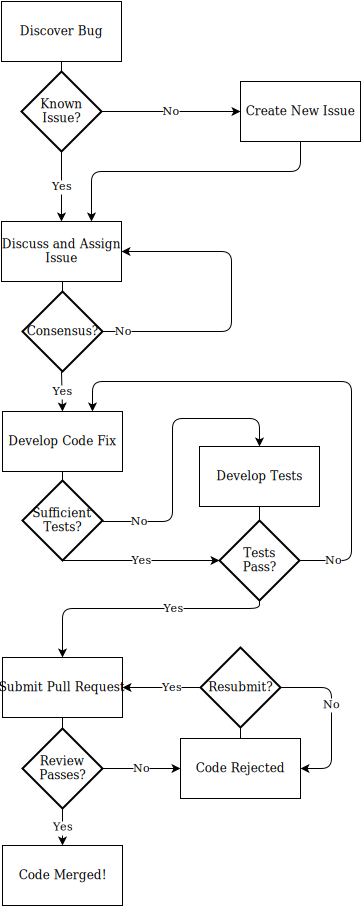
\includegraphics[height=0.6\textheight]{./images/gitprocess}
\end{center}
\caption{A version-control enabled process for finding, reporting, and fixing a bug
can take place within an issue tracker alongside multiple stages of software
testing and review. In the \Cyclus case, the final review stage includes unit,
regression, and integration testing as well as manual code inspection.}
\label{fig:gitprocess}
\end{figure}

The act of proposing a change is known as a \emph{pull request}. The main \Cyclus repository is
hosted remotely on the GitHub website \cite{dabbish_social_2012}. The online
mechanism for pull requests allows for code review by a member of the \Cyclus
core team, separate from the author, prior to any change being included. Non-members
of the \Cyclus development team are allowed and encouraged to submit and review
pull requests. However, only members of the \Cyclus core team are allowed to
merge in any changes and only after the \gls{QA} standards have been met. This
step has been repeatedly shown to improve code quality \cite{cohen_modern_2010}.

\subsubsection{Style Guide}

In any multi-person software project, there is a tension between how individuals
wish to write code. Every person tends to have their own custom style. To remedy this,
coding style guides are the software analogy to those for written language,
such as the Chicago Manual of Style. \Cyclus strictly enforces the use of the
Google C++ Style Guide \cite{weinberger_google_2008} for all software contributions.
This means that all developers of \Cyclus nominally write \Cyclus code in the same
way.  This homogenization may be a hurdle to new developers but ultimately
improves code legibility and, therefore, robustness \cite{cohen_modern_2010}.

\subsubsection{Continuous Integration}
\label{sec:qa-ci}

\emph{\acrfull{CI}} is the idea that software should be tested and validated
as it is being developed, rather than as a final stage in a longer development
cycle.  Under \gls{CI}, every pull request (proposed code change) is tested independently immediately after
it is proposed. Such tests are run on all officially supported platforms.
\Cyclus uses a \gls{CI} platform called Polyphemus
\cite{scopatz_polyphemus_2014}. Polyphemus serves as an intermediary between GitHub pull requests on the front-end
and temporary \Cyclus servers on the back-end. These servers are hosted by
the Build \& Test Laboratory (BaTLab) \cite{uw_batlab_team_batlab_2014} at the University of
Wisconsin-Madison. Whenever a pull request is created, Polyphemus performs
the following actions:

\begin{enumerate}
    \item Copies \Cyclus with the proposed new code to BaTLab,
    \item Initializes Linux and Mac OSX servers,
    \item Builds \Cyclus on all platforms,
    \item Runs the complete \Cyclus test suite,
    \item Reports whether or not the above steps succeeded.
\end{enumerate}

Since these steps are performed for all incoming code, it is easyi for the
\Cyclus core team to determine whether or not an individual pull request
actually works. This helps identify build and test problems prior to
broken code being allowed into the develop branch. \gls{CI} is a necessary
but not sufficient addition to the \Cyclus \gls{QA}
system: it keeps bad code out of \Cyclus. However, \Cyclus will always
require human eyes and hands to let good code in.
